\documentclass[11pt]{article}
\usepackage[margin=1in]{geometry}
\usepackage[T1]{fontenc}
\usepackage{lmodern}
\usepackage{microtype}
\usepackage{booktabs}
\usepackage{multirow}
\usepackage{graphicx}
\usepackage{tikz}
\usepackage{float}
\usepackage{amsmath}
\usepackage{amssymb}
\IfFileExists{siunitx.sty}{\usepackage{siunitx}}{}
\usepackage{xcolor}
\usepackage{hyperref}
\usepackage[round,authoryear]{natbib}
\hypersetup{colorlinks=true,linkcolor=blue!50!black,citecolor=blue!50!black,urlcolor=blue!50!black}

\newcommand{\AtoY}{$A\!\rightarrow\!Y$}
\newcommand{\HtoY}{$H\!\rightarrow\!Y$}
\newcommand{\AHtoY}{$[A;H]\!\rightarrow\!Y$}

\title{Emotion Categories in Frozen Transformer Representations\\[6pt]
{\large Leakage-Controlled Probing with Appraisal Residuals and Geometric Decoder Analysis}}
\author{}
\date{}

\begin{document}
\maketitle

\begin{abstract}
We ask where emotion-category labels are linearly accessible in frozen Transformer representations under a leakage-controlled protocol. On crowd-enVENT (13 writer-prompted categories, 21-dimensional appraisal ratings) and EmoTwiCS (multilabel Dutch customer-service tweets, 9 categories), we compare appraisal-to-label (\AtoY), hidden-state-to-label (\HtoY), and combined (\AHtoY) decoders with every data-dependent operation fitted inside training folds and writer/conversation-disjoint splits. Layerwise frozen probes show mid-to-late accessibility; writer appraisals add 0.28--0.47~bits of conditional held-out information beyond frozen text at the final layer (0.55--0.62~bits early, when $H$ is less informative and leaves more residual for $A$), conditional on writer-as-common-rater for $A$ and $Y$, with group-bootstrap intervals excluding zero across three encoder families; a train-fold PCA dimensionality control finds this gain largely low-rank (the top three appraisal components retain 67--77\%) yet with a statistically significant fine-grained residual through ten components, while broad VAD adds $\sim$0.06~bits on EmoTwiCS. The geometric rewriting of linear probes as power diagrams motivates a decoder-complexity ladder from nearest-centroid through multi-prototype designs; targeted diagnostics show that the multi-prototype degradation under $k$-means reflects the unsupervised estimator, not single-cell geometry, and a discriminative multi-prototype fit matches or improves on the unconstrained single-prototype decoder.
\end{abstract}

\section{Introduction}

The question is not whether emotion categories are ontologically real but where a fixed, low-capacity decoder can access their labels. We contrast three spaces: categorical $Y$, appraisal $A$ (21D writer ratings in crowd-enVENT), and frozen Transformer hidden states $H$ (768D). A fourth, valence--arousal--dominance (VAD, 3D), serves only as an EmoTwiCS auxiliary.

A linear probe is algebraically equivalent to a power diagram---a convex tessellation of the representation space \citep{aurenhammer1987power}. This geometric rewriting motivates a decoder-complexity ladder that tests which geometric restrictions suffice. The equivalence may provide a bridge to conceptual-space accounts of natural concepts \citep{gardenfors2000conceptual,douven-gardenfors-2020}, but we do not test that psychological interpretation here.

Three questions structure the investigation:
\begin{itemize}
\item[\emph{Q1.}] \emph{Accessibility:} where are emotion-category labels linearly accessible in frozen representations?
\item[\emph{Q2.}] \emph{Appraisal residual:} what do explicit appraisals contribute beyond frozen text representations, and how low-dimensional is that contribution?
\item[\emph{Q3.}] \emph{Geometry:} what geometric restrictions suffice for decoding these categories?
\end{itemize}

\citet{troiano-etal-2023-dimensional} already compared appraisal-to-emotion, text-to-emotion, and text-plus-appraisal models on crowd-enVENT with a fine-tuned encoder. Our contribution is different: we freeze every backbone parameter, resolve every layer, exclude author and duplicate leakage, nest all model selection, and quantify information rather than only accuracy. Controls (lexical, random-encoder), conditional held-out information \citep{hewitt-etal-2021-conditional}, and a geometric decoder ladder are evaluated under the same nested protocol. EmoTwiCS \citep{labat-etal-2024-emotwics,labat-etal-2022-emotional} supplies a structurally different, multilingual, multilabel setting.

We interpret probes as protocol-relative usable information \citep{xu2020theory}. Control tasks and capacity constrain interpretation \citep{hewitt-liang-2019-designing,pimentel-etal-2020-information,pimentel-etal-2020-pareto}; conditional probing asks what one representation adds beyond another \citep{hewitt-etal-2021-conditional}. Decodability does not imply causal use by the model \citep{ravichander-etal-2021-probing}.

\textbf{Contributions.} (1)~Leakage-controlled frozen layerwise accessibility across three base-scale encoders (RoBERTa, DeBERTa-v3, XLM-R) (Q1). (2)~Conditional appraisal gain of 0.28--0.47~bits beyond frozen text, with a cross-rater control, a VAD auxiliary at $\sim$0.06~bits (indirect cross-corpus), and a fold-specific PCA dimensionality control localizing most of the gain in the top three appraisal components (67--77\%) while a significant residual persists through ten components (Q2). (3)~Geometric decoder tests with targeted multi-prototype diagnostics showing that the unsupervised site estimator, not multi-prototype geometry, drives the multi-prototype degradation: centroid anchoring does not recover it, while a discriminative multi-prototype fit eliminates it and, on appraisals, significantly improves on the single-prototype power diagram (Q3).

\section{Data and leakage-controlled protocol}
\label{sec:protocol}

\subsection{Corpora}

crowd-enVENT\footnote{\url{https://www.romanklinger.de/data-sets/crowd-enVent2023.zip}} comprises generation texts with writer labels $Y_{\mathrm{writer}}$ (13 categories) and writer appraisals $A_{\mathrm{writer}}$ (21D), plus a validated subset with five independent reader judgments per text (Table~\ref{tab:audit}). $Y_{\mathrm{writer}}$ is a prompted self-report, not a discovered natural kind. Validated items yield $Y_{\text{reader majority}}$ and the empirical five-reader distribution as separate outcomes. Writer and reader appraisals are never conflated; split-panel analyses that use disjoint readers for coordinates and labels are exploratory and high-variance. EmoTwiCS\footnote{\url{https://lt3.ugent.be/resources/emotwics/}} contains customer tweets grouped by conversation, multilabel over nine documented clusters, with 3D VAD retained only as an auxiliary.

\begin{table}[h]
\centering\small
\begin{tabular}{lr}
\toprule
Analysis unit & Count \\
\midrule
crowd-enVENT generation items & 6,600 \\
Writers & 2,379 \\
Validated items (5 judgments each) & 1,200 \\
EmoTwiCS conversations & $\sim$9.5k \\
EmoTwiCS customer tweets & $\sim$13.2k \\
\bottomrule
\end{tabular}
\caption{Corpus scale. Validated items are fully disjoint from training writers and normalized text duplicates in held-out evaluation.}
\label{tab:audit}
\end{table}

No claim about natural-kind status is made; labels index linearly accessible structure under the stated protocol.

\subsection{Leakage-controlled evaluation}

All data-dependent operations---per-coordinate standardization, block scaling, optional PCA, vocabulary/IDF, calibration, regularization, and multilabel thresholds---are fitted on training folds only. Test labels never select a layer, pooling rule, masking, block weight, class subset, or threshold. Item-level out-of-fold probabilities are the sole source of metrics (accuracy, macro-F1, log loss in bits, ECE, Brier), reconstructed per item to preserve pairing.

Splits are group-aware: connected components of writer (crowd-enVENT) or conversation (EmoTwiCS) plus normalized duplicate texts define groups. Evaluation uses five outer folds and three inner folds for hyperparameter selection (regularization strength $C$, and for EmoTwiCS a global threshold). Inner selection optimizes held-out log loss (or macro-F1 where noted). A sealed validated partition is held out as an external test and never informs any selection. The same outer/inner splits are reused across every representation and decoder so that paired $\Delta L$ is well-defined itemwise. Group-bootstrap intervals preserve writer/conversation dependence.

The reported group-bootstrap intervals have nominal 95\% coverage for their individual paired contrasts; no simultaneous, across-table multiplicity adjustment is claimed. They are therefore per-contrast uncertainty statements, not a global pass/fail criterion.

The same protocol applies to lexical and control baselines, so differences cannot be attributed to leakage or selection asymmetry.

\subsection{Frozen representations and probes}

Primary English encoders are RoBERTa-base \citep{liu-etal-2019-roberta} and DeBERTa-v3-base \citep{he-etal-2021-debertav3}; XLM-RoBERTa-base \citep{conneau-etal-2020-unsupervised} is used across languages. All backbone parameters are frozen; inference uses attention-mask-aware mean pooling over non-special content tokens. Sensitivities include first-token pooling and masking of direct emotion expressions. Representations are denoted $H_{\ell}$ for layer $\ell\in\{0,\dots,12\}$.

The multiclass probe is $L_{2}$-regularized multinomial logistic regression on standardized inputs; the multilabel probe is $L_{2}$-regularized one-vs-rest logistic regression. Regularization $C$ (and the EmoTwiCS global threshold) is chosen in the inner fold. A linear SVM is used only for margin diagnostics. Random encoders reuse the same architecture and tokenizer with a frozen random initialization and test for token-identity/architecture effects, not classifier chance.

\section{Layerwise linear accessibility}
\label{sec:layerwise}

Figure~\ref{fig:layerwise} shows layerwise probing. Panel~(a) is crowd-enVENT macro-F1 by layer under writer-disjoint nested selection; panel~(b) is EmoTwiCS XLM-R confirmatory macro-F1/AP with the TF--IDF reference (0.464). Each point is test-independent with its own inner-fold $C$.

\begin{figure}[t]
\centering
\begin{minipage}{0.49\textwidth}
\centering
\includegraphics[width=\textwidth]{results/figures/layerwise_crowd.pdf}
{\footnotesize (a) crowd-enVENT (13-way).}
\end{minipage}\hfill
\begin{minipage}{0.49\textwidth}
\centering
\includegraphics[width=\textwidth]{results/figures/layerwise_emotwics.pdf}
{\footnotesize (b) EmoTwiCS (XLM-R, 9 confirmatory clusters); dashed = TF--IDF.}
\end{minipage}
\caption{Layerwise frozen probing. (a) crowd-enVENT writer-label macro-F1 by layer; (b) EmoTwiCS confirmatory macro-F1/AP by layer. Both use test-independent inner-fold regularization; lines join layers only to show the trajectory. Masked mean pooling (crowd) / tweet mean pooling (EmoTwiCS). EmoTwiCS XLM-R L12 confirmatory macro-F1 = 0.455 vs.\ TF--IDF = 0.464 (Table~\ref{tab:emotwics-layer}); the TF--IDF line in (b) marks parity.}
\label{fig:layerwise}
\end{figure}

\begin{table}[h]
\centering\footnotesize
\begin{tabular}{lcc}
\toprule
EmoTwiCS (XLM-R, tweet mean) & Conf.\ macro-F1 & Macro-AP \\
\midrule
L0 & 0.425 & 0.420 \\
L6 & 0.461 & 0.449 \\
L9 (peak AP) & 0.462 & 0.458 \\
L10 (peak F1) & 0.465 & 0.457 \\
L12 & 0.455 & 0.443 \\
TF--IDF & 0.464 & 0.446 \\
Random L12 & 0.323 & 0.305 \\
\bottomrule
\end{tabular}
\caption{EmoTwiCS layerwise summary (OOF, 5-fold conversation-disjoint, full $N=13{,}172$; 9 confirmatory clusters). TF--IDF (0.464) vs.\ XLM-R L12 (0.455) parity constrains strong lexical claims on this corpus. Full 0--12 trajectory in Fig.~\ref{fig:layerwise}b; data and protocol in \S\ref{sec:protocol}.}
\label{tab:emotwics-layer}
\end{table}

Accessibility rises steeply from the embedding layer, plateaus mid-to-late, and differs slightly in peak location by family: RoBERTa-base peaks at L11 (macro-F1~0.54, log loss~2.02~bits), DeBERTa-v3-base at L9 (F1~0.56, log loss~1.98~bits), XLM-RoBERTa-base at L9 (F1~0.47, log loss~2.28~bits) under the full-generation OOF protocol. Normalized depth shows the same ordering. EmoTwiCS with XLM-R shows a comparable mid-to-late rise in confirmatory macro-F1 (Fig.~\ref{fig:layerwise}b, Table~\ref{tab:emotwics-layer}; peak L10~0.465, L12~0.455), tracking the TF--IDF reference (Fig.~\ref{fig:layerwise}b dashed; TF--IDF~0.464).

\textbf{Controls.} Under the identical protocol, TF--IDF reaches macro-F1~0.44 (full-OOF) and 0.38 (external) on crowd-enVENT, NRC lexicon $\sim$0.15, surface $\sim$0.07--0.09, prior $\sim$0.01--0.04, compared with frozen final-layer 0.46--0.53 (full-OOF) and 0.41--0.51 (external). Random encoders (L12: 0.28--0.30 full-OOF, 0.23--0.24 external) remain substantially below trained encoders, ruling out random-projection explanations. Unmasked text exceeds masked by $\sim$0.06--0.11~F1; first-token pooling underperforms mean pooling. On EmoTwiCS, TF--IDF (0.464) is on par with frozen XLM-R at L12 (0.455; Table~\ref{tab:emotwics-layer}, Fig.~\ref{fig:layerwise}b dashed), constraining strong claims on that corpus, but the crowd-enVENT lexical gap is robust (Table~\ref{tab:emotwics-layer}).

\section{Conditional appraisal information}
\label{sec:conditional}

\subsection{Conditional gain beyond frozen text}

For each outer slice we compare paired item probabilities from \HtoY\ and \AHtoY. Positive $\Delta L = L(H)-L([A;H])$ means writer appraisals reduce predictive loss beyond frozen text. Block standardization and a train-fitted appraisal multiplier prevent the larger hidden block from dominating by dimension alone. Capacity-matched sensitivities (PCA on $H$ to 21, 42, 84~D) confirm gains are not a pure dimensionality effect.

\begin{table}[h]
\centering\footnotesize
\begin{tabular}{lcccc}
\toprule
Model (design) & $\Delta L$ (bits) & $\Delta$Brier & $\Delta$F1 & $\Delta$ECE \\
\midrule
DeBERTa-v3 (OOF) & 0.34 [0.31, 0.36] & 0.065 & 0.061 & --0.013 \\
DeBERTa-v3 (external) & 0.37 [0.32, 0.44] & 0.066 & 0.080 & --0.016 \\
RoBERTa (OOF) & 0.28 [0.25, 0.30] & 0.054 & 0.050 & 0.009 \\
RoBERTa (external) & 0.32 [0.27, 0.38] & 0.062 & 0.064 & --0.012 \\
XLM-R (OOF) & 0.46 [0.41, 0.48] & 0.089 & 0.079 & 0.005 \\
XLM-R (external) & 0.47 [0.40, 0.55] & 0.092 & 0.103 & 0.026 \\
\bottomrule
\end{tabular}
\caption{Paired conditional gain of $[A;H_{12}]$ over $H_{12}$-only (bits/item, $H-AH$). Intervals are group-bootstrap 95\% CIs preserving writer dependence. Positive $\Delta L$/$\Delta$F1 = appraisals help beyond text. L12 is reported here; the layerwise gain trajectory is summarized in the text below.}
\label{tab:conditional}
\end{table}

At the final layer (L12, Table~\ref{tab:conditional}), conditional log-loss gains are 0.28--0.46~bits (OOF) and 0.32--0.47~bits (external) with intervals excluding zero in all six family-by-design cells; macro-F1 gains are 0.05--0.10 and Brier improvements 0.05--0.09. Classwise, gains are largest for joy, guilt, and anger ($>$0.5~bits) and smallest for boredom and disgust. Layerwise, $\Delta L$ shrinks as $H$ becomes more informative (L0: $\sim$0.55--0.62~bits; L6: $\sim$0.31--0.47~bits; L12: $\sim$0.28--0.46~bits) but remains positive at every layer.

The $\Delta$ECE entries are binned calibration diagnostics rather than the optimized log-loss, so they need not move in the same direction. ECE improves in three cells but increases modestly in RoBERTa OOF and both XLM-R cells despite their gains in log loss and macro-F1.

\subsection{Dimensionality of the appraisal residual}

To test whether the conditional gain lives in a few dominant appraisal directions or is distributed across the full 21-dimensional space, we compress the appraisal block to its top $d\in\{3,5,7,10\}$ principal components. PCA is refit on each outer training fold only (inside the estimator, so no outer-test appraisal contributes), with block standardization, inner-fold $C$, and appraisal-multiplier selection unchanged from the full-21D pipeline. Table~\ref{tab:pca-dims} reports $\Delta L_{d}=L(H)-L([A_{\mathrm{PCA}\text{-}d};H_{12}])$ with 2{,}000 paired writer-group bootstrap resamples, together with the direct paired contrast against the full block. The top three components already recover 67--77\% of the full-21D gain per encoder, so most of the appraisal contribution is low-rank. However, the paired contrast $\Delta\Delta L_{d}=\Delta L_{d}-\Delta L_{21}$ remains significantly negative at every $d$ and for every encoder: even $d=10$ loses 0.03--0.05~bits (intervals $[-0.06,-0.02]$), and appraisal-only probing degrades monotonically from 2.48~bits (full 21D) through 2.56~bits ($d{=}10$) to 2.78~bits ($d{=}3$). The appraisal residual beyond frozen text thus concentrates in the dominant appraisal directions \emph{and} retains a small but real fine-grained component that the leading components do not restore.

\begin{table}[h]
\centering\footnotesize
\begin{tabular}{ccccc}
\toprule
$d$ & DeBERTa-v3 & RoBERTa & XLM-R & $\Delta\Delta L$ vs 21D (range) \\
\midrule
3 & 0.24 [0.22, 0.26] & 0.21 [0.20, 0.23] & 0.31 [0.28, 0.33] & $-0.06$ to $-0.15$ \\
5 & 0.28 [0.25, 0.30] & 0.24 [0.22, 0.26] & 0.36 [0.32, 0.39] & $-0.04$ to $-0.10$ \\
7 & 0.29 [0.27, 0.32] & 0.25 [0.23, 0.27] & 0.39 [0.36, 0.43] & $-0.03$ to $-0.06$ \\
10 & 0.31 [0.28, 0.33] & 0.25 [0.22, 0.27] & 0.41 [0.37, 0.44] & $-0.03$ to $-0.05$ \\
\midrule
21 (full) & 0.34 [0.31, 0.37] & 0.28 [0.25, 0.31] & 0.45 [0.42, 0.49] & 0 \\
\bottomrule
\end{tabular}
\caption{Dimensionality control of the appraisal block (full-OOF, L12). $\Delta L_{d}$ is the paired conditional gain of $[A_{\mathrm{PCA}\text{-}d};H_{12}]$ over $H_{12}$-only in bits/item; PCA is refit inside each outer training fold. Brackets: paired writer-group bootstrap 95\% CIs (2{,}000 resamples). Last column: range over encoders of the direct paired contrast $\Delta L_{d}-\Delta L_{21}$ (negative = information lost to compression); every cell's interval excludes zero.}
\label{tab:pca-dims}
\end{table}

\begin{figure}[t]
\centering
\includegraphics[width=.88\textwidth]{results/figures/conditional_gain.pdf}
\caption{Conditional log-loss gain $\Delta L$ with group-bootstrap intervals. Dashed line = no gain. All intervals exclude zero.}
\label{fig:cond}
\end{figure}

\textbf{What do the dominant components represent?}
To interpret the low-rank structure, Table~\ref{tab:pca-loadings} reports the five highest-magnitude PCA loadings for each of the first three components.
Loadings are averaged across the five outer-fold PCA fits (sign-aligned to the full-sample solution); cross-fold cosine similarity exceeds 0.999 for PC1 and averages $\sim$0.95 for PC2 and PC3, indicating stable axes.

\begin{table}[h]
\centering\footnotesize
\begin{tabular}{clr@{\hskip 6pt}clr@{\hskip 6pt}clr}
\toprule
\multicolumn{3}{c}{PC1 (23.0\%)} & \multicolumn{3}{c}{PC2 (10.9\%)} & \multicolumn{3}{c}{PC3 (10.5\%)} \\
\midrule
$+$ & unpleasantness & .37 & $+$ & urgency & .35 & $+$ & effort & .36 \\
$+$ & standards & .30 & $+$ & attention & .34 & $+$ & predict\_conseq & .36 \\
$-$ & pleasantness & .35 & $+$ & goal\_relevance & .31 & $+$ & attention & .33 \\
$-$ & goal\_support & .31 & $-$ & familiarity & .31 & $+$ & self\_control & .30 \\
$+$ & not\_consider & .29 & $-$ & predict\_event & .29 & $+$ & self\_responsblt & .28 \\
\bottomrule
\end{tabular}
\caption{Top-five PCA loadings per component (absolute value shown; sign column indicates direction). Names, including \texttt{self\_responsblt}, are verbatim crowd-enVENT field names. Loadings are fold-averaged ($\pm\!\le\!0.01$ for PC1; $\le\!0.07$ for PC2--3). The three components account for 44.4\% of appraisal variance but 67--77\% of the conditional predictive gain beyond frozen text.}
\label{tab:pca-loadings}
\end{table}

PC1 loads positively on \emph{unpleasantness}, \emph{standards}, \emph{social\_norms}, and \emph{not\_consider}, and negatively on \emph{pleasantness} and \emph{goal\_support}: it correlates $r=-0.81$ with a pleasantness$\,-\,$unpleasantness proxy, identifying it as a valence axis enriched with normative appraisals (moral transgression, social expectation).
PC2 loads on \emph{urgency}, \emph{attention}, and \emph{goal\_relevance} against \emph{familiarity} and \emph{predict\_event}: an arousal/novelty axis capturing whether the event is salient, unfamiliar, and demands immediate processing.
PC3 loads on \emph{effort}, \emph{predict\_conseq}, \emph{self\_control}, and \emph{self\_responsblt}: an agency/coping-potential axis reflecting the writer's perceived ability and willingness to act on the situation.
These three axes overlap with, but do not reduce to, classical VAD: PC1 carries a normative component absent from a pure hedonic-valence dimension, and PC3 is closer to coping potential than to generic dominance.
The concentration of conditional information in the leading components is compatible with longstanding evidence that a small number of broad appraisal dimensions discriminate major emotion categories \citep{scherer1997profiles,fontaine-etal-2007-two-dimensional}.
The significant residual beyond them is equally expected: componential analyses recover additional factors for novelty, expectancy, coping, goal relevance, norm violation, and causal agency \citep{fontaine-scherer-2013}, and a meta-analysis of 309 studies assessing 47 appraisal dimensions and 63 emotions documents a substantially richer appraisal--emotion association structure \citep{yeo-ong-2024}.
The alignment with appraisal-theoretic constructs suggests that the dominant residual information beyond frozen text is not an artefact of scale covariance but tracks psychologically interpretable dimensions.

\subsection{Cross-rater control}
\label{sec:crossrater}

The primary comparison uses $A_{\mathrm{writer}}$ and $Y_{\mathrm{writer}}$ from the same respondent, conflating text-unexpressed appraisal content with consistency in scale use and private context. To partially disentangle these, we evaluate probes on the 1{,}200 validated items with writer appraisals predicting \emph{reader}-majority labels ($A_{\mathrm{writer}}\!\rightarrow\!Y_{\mathrm{reader}}$), eliminating rater overlap between the appraisal coordinates and the target. Writer appraisals still add 0.14--0.21~bits beyond $H$ for predicting reader labels across all three encoders (Appendix~\ref{app:reader}, Table~\ref{tab:reader}), demonstrating that the appraisal gain is not entirely attributable to common-rater method variance. An adequately powered $A_{\mathrm{reader}}\!\to\!Y_{\mathrm{reader}}$ design with disjoint, larger reader panels remains the priority for a definitive test.

\subsection{Auxiliary comparison with 3D VAD}
\label{sec:vad}

On EmoTwiCS (XLM-R, same nested splits), adding 3D VAD to $H$ improves held-out binary cross-entropy by only $0.06$~bits at L12 (0.07~bits at L0; $\Delta$F1 $\sim$0.10), versus 0.28--0.47~bits (final) and 0.55--0.62~bits (early) for 21D appraisals beyond $H$ on crowd-enVENT (Table summarised in text). The VAD residual is an order of magnitude smaller than the 21D appraisal residual, but the comparison is indirect: corpora differ in language, label set (9 vs.\ 13), task (multilabel vs.\ multiclass), and annotation protocol. Whether the difference reflects the richer representational capacity of appraisals or these confounding factors requires a within-corpus test with both VAD and 21D appraisals on the same items.

\section{Geometric decoder tests}
\label{sec:ladder}

\subsection{Power diagrams and linear probes}

\paragraph{From Voronoi to power diagrams.}
Consider first $K$ sites $p_1,\ldots,p_K$ in a Euclidean representation space. An ordinary Voronoi diagram assigns a point $z$ to the site to which it is closest:
\begin{equation}
V_k=\left\{z:\|z-p_k\|^2\leq\|z-p_j\|^2\quad\forall j\right\}. \label{eq:vorcell}
\end{equation}
Each pairwise boundary is therefore the perpendicular bisector of the corresponding pair of sites (Figure~\ref{fig:voronoi-power}a).

A power diagram (or Laguerre--Voronoi tessellation) \citep{aurenhammer1987power} augments each site $p_k$ with a scalar weight $\omega_k$ and replaces squared Euclidean distance by the \emph{power distance} (itself not a metric: it can be negative and satisfies no triangle inequality)
\begin{equation}
\pi_k(z)=\|z-p_k\|^2-\omega_k. \label{eq:powerdist}
\end{equation}
The cell associated with site $k$ is
\begin{equation}
P_k=\left\{z:\pi_k(z)\leq\pi_j(z)\quad\forall j\right\}. \label{eq:powcell}
\end{equation}
Thus $\omega_k$ acts as a site-specific additive advantage: increasing $\omega_k$ lowers the score of site $k$ uniformly over the space and can expand its cell. Ordinary Voronoi diagrams are the special case in which all $\omega_k$ are equal (in particular, all zero); only weight differences matter, since adding a common constant to all $\omega_k$ leaves the partition unchanged. The decoder ladder of \S\ref{sec:ladder-defs} tests this passage both at fixed sites (D1$\to$D1o) and with re-fitted sites (D2$\to$D3), where a gauge equivalence makes the two predictive classes coincide (see \S\ref{sec:ladder-defs}).\footnote{When $\omega_k\geq0$, one may write $\omega_k=r_k^2$ and interpret the construction through the classical power of a point with respect to spheres of radius $r_k$, hence the name \emph{power diagram}. The representation is non-canonical, however, because the partition is invariant under $(\omega_1,\dots,\omega_K)\mapsto(\omega_1+c,\dots,\omega_K+c)$, so infinitely many radius collections yield the same diagram. We therefore prefer the additive-advantage interpretation in the main text.}

For two sites $p_i$ and $p_j$, their power boundary satisfies
\begin{equation}
2(p_j-p_i)^\top z=\|p_j\|^2-\|p_i\|^2+\omega_i-\omega_j. \label{eq:pairwise}
\end{equation}
Hence weighting does not arbitrarily rotate or curve a Voronoi boundary: it translates the separating hyperplane while preserving its normal direction $p_j-p_i$. If $\omega_i=\omega_j$ this is exactly the perpendicular bisector; if $\omega_i>\omega_j$ the boundary moves toward $p_j$ and the cell of $i$ grows. Relative to the ordinary Voronoi bisector, the signed displacement, measured along the unit direction $(p_j-p_i)/\|p_j-p_i\|$, is
\begin{equation}
\delta_{ij}=\frac{\omega_i-\omega_j}{2\|p_i-p_j\|}, \label{eq:disp}
\end{equation}
so $\delta_{ij}>0$ means the bisector has shifted toward $p_j$.
Power diagrams therefore generalize Voronoi diagrams while retaining convex polyhedral cells and affine pairwise boundaries: power weighting adds flexibility without allowing arbitrary decision surfaces (Figure~\ref{fig:voronoi-power}b).

\begin{figure}[H]
\centering
\begin{minipage}[t]{0.48\textwidth}
\centering
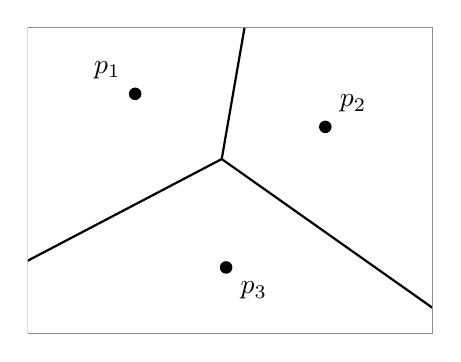
\begin{tikzpicture}[scale=1.05,
  site/.style={circle,fill,inner sep=1.6pt},
  bnd/.style={thick}]
  \clip (-1.3,-1.8) rectangle (3.6,1.9);
  % Voronoi boundaries from vertex v=(1.047,0.311)
  \draw[bnd] (1.047,0.311) -- (1.323,1.9);
  \draw[bnd] (1.047,0.311) -- (-1.3,-0.919);
  \draw[bnd] (1.047,0.311) -- (3.6,-1.491);
  % sites
  \node[site,label=above left:{$p_1$}] at (0,1.1) {};
  \node[site,label=above right:{$p_2$}] at (2.3,0.7) {};
  \node[site,label=below right:{$p_3$}] at (1.1,-1.0) {};
  % discrete frame
  \draw[black!45,thin] (-1.3,-1.8) rectangle (3.6,1.9);
\end{tikzpicture}\\[2pt]
{\footnotesize (a) Ordinary Voronoi ($\omega_1=\omega_2=\omega_3$)}
\end{minipage}\hfill
\begin{minipage}[t]{0.48\textwidth}
\centering
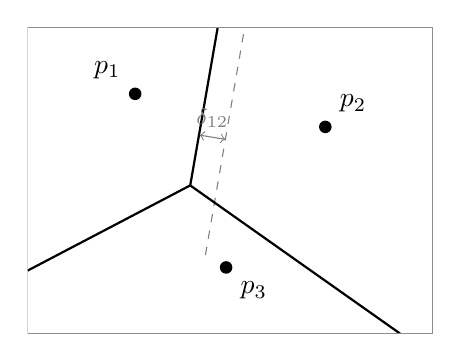
\begin{tikzpicture}[scale=1.05,
  site/.style={circle,fill,inner sep=1.6pt},
  bnd/.style={thick}]
  \clip (-1.3,-1.8) rectangle (3.6,1.9);
  % old Voronoi bisector of (p1,p2), dashed
  \draw[dashed,gray] (0.85,-0.85) -- (1.324,1.9);
  % power boundaries from vertex v'=(0.666,-0.008)
  \draw[bnd] (0.666,-0.008) -- (0.998,1.9);
  \draw[bnd] (0.666,-0.008) -- (-1.3,-1.038);
  \draw[bnd] (0.666,-0.008) -- (3.204,-1.8);
  % displacement arrow between old bisector and power boundary
  \draw[<->,gray] (1.09,0.55) -- (0.78,0.60)
    node[midway,above,font=\footnotesize] {$\delta_{12}$};
  % sites
  \node[site,label=above left:{$p_1$}] at (0,1.1) {};
  \node[site,label=above right:{$p_2$}] at (2.3,0.7) {};
  \node[site,label=below right:{$p_3$}] at (1.1,-1.0) {};
  % discrete frame
  \draw[black!45,thin] (-1.3,-1.8) rectangle (3.6,1.9);
\end{tikzpicture}\\[2pt]
{\footnotesize (b) Power diagram ($\omega_1{=}0,\ \omega_2{=}1.5,\ \omega_3{=}{-}0.5$)}
\end{minipage}
\caption{Same three sites under (a) an ordinary Voronoi diagram and (b) a power diagram. Weighting translates each pairwise boundary parallel to itself while preserving its normal direction $p_j-p_i$; the dashed line is the original Voronoi bisector of $(p_1,p_2)$ and $\delta_{12}$ is the signed displacement of \eqref{eq:disp}. Because $\omega_2>\omega_1$, the boundary moves toward $p_1$ and cell $P_2$ expands.}
\label{fig:voronoi-power}
\end{figure}

\paragraph{Equivalence with a multiclass linear probe.}
Let $z = T_{\mathrm{train}}(x)\in\mathbb{R}^{D}$ be the representation after preprocessing fitted only on the training fold (standardization; optional PCA). The multiclass linear probe predicts
\begin{equation}
\hat y(z)=\arg\max_{k}\,(w_{k}^{\top}z+b_{k}). \label{eq:linear}
\end{equation}
Writing $\|z-p_{k}\|^{2}-\omega_{k}=\|z\|^{2}-w_{k}^{\top}z-b_{k}$ with
\begin{equation}
p_{k}=w_{k}/2,\qquad \omega_{k}=b_{k}+\|w_{k}\|^{2}/4, \label{eq:pow}
\end{equation}
and noting $\|z\|^{2}$ is common to all $k$,
\begin{equation}
\hat y(z)=\arg\min_{k}\{\|z-p_{k}\|^{2}-\omega_{k}\}. \label{eq:voronoi}
\end{equation}
Equation~\eqref{eq:voronoi} is exactly the power-diagram assignment rule of \eqref{eq:powcell} with sites and weights given by \eqref{eq:pow}: every multiclass linear probe induces a power diagram in the preprocessed coordinate system, and conversely. Each class region is a (possibly empty) convex polyhedron; boundaries are hyperplanes. The equivalence is algebraic, not evidence that categories are psychologically convex or prototype-based \citep{gardenfors2000conceptual}. This geometric formulation may provide a bridge to conceptual-space accounts that identify natural concepts with convex regions \citep{gardenfors2000conceptual,douven-gardenfors-2020}, but we do not test that psychological interpretation here.
Two caveats are essential. First, preprocessing-relativity: Euclidean distance in $z$ equals a diagonal Mahalanobis distance (plus rotation if PCA is applied) in raw coordinates, so no Euclidean metric in raw appraisal or hidden space is identified. Second, identification: softmax scores are invariant to adding a common affine function to every class, so absolute sites $p_{k}$ are convention-dependent (e.g.\ $\sum_{k}w_{k}=0$); invariant quantities are pairwise boundaries $w_{k}-w_{j}$, offsets $b_{k}-b_{j}$, and cell adjacencies. Sites are discriminative parameters, not empirical centroids, and not psychological prototypes absent similarity/typicality validation \citep{nosofsky1986attention,shepard1987toward}.
\subsection{Nested geometric restrictions}
\label{sec:ladder-defs}

We evaluate decoders on the \emph{same} frozen $z$ and the \emph{same} outer/inner split lock as \S\S\ref{sec:layerwise}--\ref{sec:conditional}, differing only in which geometric parameters are fitted: prior-only (D0), nearest centroid (D1), centroid-offset diagram (D1o: D1 centroids frozen, free per-class offsets $\omega_k$, shared scale $\gamma$), ordinary Voronoi (D2, single site/class, tied $\omega$), power diagram (D3, single site/class, free $\omega_{k}$---equivalent to unconstrained logistic regression via \eqref{eq:pow}), and multi-prototype (D4, $m=2$--$3$ sites/class). D1 converts squared-distance scores to probabilities through $\operatorname{softmax}(-\gamma d_k^2)$; D1o uses $\operatorname{softmax}_k(-\gamma\|z-c_k\|^2+\omega_k)$, keeping the sites $c_k$ fixed at the D1 centroids and learning only the free offsets $\omega_k$. In D1/D1o, $\gamma$ leaves hard nearest-site assignments unchanged but calibrates the held-out log loss. The multi-prototype family (D4, D4c, D4d) shares one class-scoring rule: the class score is the log-sum-exp over its $m$ sites of $\omega_{kj}-\gamma\|z-p_{kj}\|^{2}$, with probabilities obtained by softmax over classes. D4 and D4c fit sites by per-class $k$-means (D4c freezing one site at the class centroid) with $\omega_{kj}=0$ and $\gamma$ selected on inner folds; D4d refines the same initialisation by L-BFGS on the multiclass cross-entropy, fitting both sites and per-site weights $\omega_{kj}$ (with $\gamma$ absorbed into the sites) under a penalty matching D3's ridge on the effective linear-probe parameters, so $m{=}1$ recovers D3 exactly. In every decoder, $\gamma$, $m\in\{2,3\}$, and the regularisation strength $C$ are selected on inner folds (Table~\ref{tab:ladder}). D1$\to$D1o quantifies \emph{offset need} at fixed prototype geometry. Two diagnostic variants extend D4 (\S\ref{sec:ladder}): centroid-anchored $k$-means (D4c) and the discriminative refinement (D4d). All are CPU-only $L$-BFGS / $k$-means fits.\footnote{A shared-Mahalanobis power diagram with metric $M$, free sites $p_k$, and free offsets $\omega_k$ assigns class scores $-(z-p_k)^\top\!M(z-p_k)+\omega_k$. Because the quadratic term $z^\top\!Mz$ is common to all $k$, the decision rule reduces to $\arg\max_k\,(2p_k^\top\!Mz - p_k^\top\!Mp_k + \omega_k)$, which is affine in $z$---algebraically equivalent to D3. Introducing $M$ therefore changes the parametrisation, not the class of realisable decision boundaries.}

Because the softmax gauge freedom $(w_k,b_k)\mapsto(w_k+a,\,b_k+c)$ acts on the power representation as $p_k\mapsto p_k+a/2$ and $\omega_k\mapsto\omega_k+c+\tfrac12 w_k^\top a+\tfrac14\|a\|^2$, any fitted D3 diagram can be re-expressed as an ordinary Voronoi diagram with identical probabilities whenever the linear system $(w_k-w_1)^\top a=-2(b_k-b_1)-\tfrac12(\|w_k\|^2-\|w_1\|^2)$, $k=2,\dots,K$, admits a solution. This is a $(K-1)\times D$ system. For every fitted D3 solution in the present experiments, the $((K-1)\times D)$ weight-difference matrix has full row rank $K-1$ (verified on every fold of both spaces), so an exactly prediction-equivalent ordinary-Voronoi reparametrisation exists. Thus the observed D2/D3 gap reflects ridge and optimisation differences between the two parametrisations rather than a need for offsets.

\begin{table}[t]
\centering\footnotesize
\caption{Decoder ladder on crowd-enVENT (5 outer / 3 inner group-aware folds; $T_{\mathrm{train}}$ fitted train-only; distance scale $\gamma$, multi-prototype count $m\in\{2,3\}$, and regularisation $C$ selected on inner folds). Log loss is held-out cross-entropy; code length $\approx N\!\times\!L$. $\Delta$ vs.\ prior is negative when saving bits. D2--D3 gap (bits) reflects the residual between tied- and free-$\omega$ parametrisations under the gauge equivalence discussed in the text. $N=6600$, $K=13$. Shared-Mahalanobis variants are algebraically equivalent to D3 in decision boundaries (see footnote in text) and omitted.}
\label{tab:ladder}
\resizebox{\textwidth}{!}{%
\begin{tabular}{lccccc}
\toprule
Decoder & $L$ (nats) & $L$ (bits) & Total (kbits) & $\Delta$ vs prior (bits) & D2--D3 gap (bits) \\
\midrule
\multicolumn{6}{c}{\textit{Appraisal $A$ 21D (standardized)}} \\
Prior-only (D0) & $2.544\pm0.005$ & $3.671\pm0.007$ & 24.23 & 0.000 & -- \\
Nearest-centroid (D1) & $1.883\pm0.035$ & $2.717\pm0.051$ & 17.93 & --0.953 & -- \\
Centroid-offset (D1o) & $1.870\pm0.038$ & $2.698\pm0.055$ & 17.81 & --0.973 & -- \\
Learned Voronoi (D2) & $1.719\pm0.039$ & $2.480\pm0.057$ & 16.37 & --1.191 & \multirow{2}{*}{0.002} \\
Power diagram (D3) & $1.717\pm0.035$ & $2.478\pm0.051$ & 16.35 & --1.193 & \\
Multi-prototype $k$-means (D4, $m=2$--$3$) & $1.791\pm0.035$ & $2.583\pm0.051$ & 17.05 & --1.088 & -- \\
\quad centroid-anchored (D4c) & $1.862\pm0.039$ & $2.687\pm0.057$ & 17.73 & --0.984 & -- \\
\quad discriminative refinement (D4d) & $1.691\pm0.031$ & $2.439\pm0.045$ & 16.10 & --1.232 & -- \\
\midrule
\multicolumn{6}{c}{\textit{Frozen $H$ RoBERTa L12, 768D $\to$ PCA 64 (train-only)}} \\
Prior-only (D0) & $2.544\pm0.005$ & $3.671\pm0.007$ & 24.23 & 0.000 & -- \\
Nearest-centroid (D1) & $1.796\pm0.043$ & $2.591\pm0.061$ & 17.10 & --1.079 & -- \\
Centroid-offset (D1o) & $1.780\pm0.044$ & $2.569\pm0.063$ & 16.95 & --1.102 & -- \\
Learned Voronoi (D2) & $1.541\pm0.059$ & $2.224\pm0.086$ & 14.68 & --1.447 & \multirow{2}{*}{0.026} \\
Power diagram (D3) & $1.523\pm0.056$ & $2.197\pm0.081$ & 14.50 & --1.473 & \\
Multi-prototype $k$-means (D4, $m=2$--$3$) & $1.896\pm0.055$ & $2.736\pm0.079$ & 18.06 & --0.935 & -- \\
\quad centroid-anchored (D4c) & $2.177\pm0.094$ & $3.141\pm0.135$ & 20.73 & --0.530 & -- \\
\quad discriminative refinement (D4d) & $1.524\pm0.058$ & $2.199\pm0.084$ & 14.51 & --1.472 & -- \\
\bottomrule
\end{tabular}%
}
\end{table}

\subsection{Results}

\textbf{D2 $\approx$ D3 is a parametrisation equivalence, not evidence that offsets are unneeded.} For $A$ 21D, D2--D3 differ by $0.002$~bits/label; for $H$ PCA64, by $0.026$~bits (Table~\ref{tab:ladder}). This is expected: under the softmax gauge, every fitted D3 solution in the present experiments has a weight-difference matrix of full row rank $K-1=12$, and therefore admits an prediction-equivalent ordinary-Voronoi reparametrisation (\S\ref{sec:ladder-defs}). The residual gap reflects ridge regularisation and L-BFGS convergence differences between tied-$\omega$ and free-$\omega$ parametrisations, not a structural need for offsets. The clean test of offset need fixes the sites and compares D1 to D1o: on $A$ 21D, freeing the offsets at frozen centroids improves held-out loss by $0.019$~bits (95\% CI $[-0.026, -0.013]$); on $H$ PCA64, by $0.023$~bits (95\% CI $[-0.029, -0.017]$), confirming that offsets contribute marginally when prototype locations are held fixed. Allowing the sites themselves to move (D1o$\to$D3) yields a substantially larger improvement: $0.220$~bits on $A$ (95\% CI $[0.197, 0.243]$), $0.371$~bits on $H$ (95\% CI $[0.345, 0.397]$).

\textbf{Multi-prototype $k$-means degrades relative to D3.} Under matched inner-fold calibration of $\gamma$ (Table~\ref{tab:ladder}), D4 ($m=2$--$3$ per class, $k$-means with 5 restarts, soft log-sum-exp site aggregation) \emph{increases} held-out code length relative to D3 by $+0.106$~bits on $A$ (paired group-bootstrap 95\% CI $[0.085, 0.126]$) and $+0.538$~bits on $H$ (95\% CI $[0.503, 0.572]$). In the hidden-state space it is additionally worse than D1 ($2.736$ vs.\ $2.591$~bits, 95\% CI for $\Delta$~$[0.120, 0.168]$); in the appraisal space it improves on D1 ($2.583$ vs.\ $2.717$~bits, 95\% CI for $\Delta$~$[-0.162, -0.106]$), so the D4/D1 ordering is space-dependent. The robust finding is the degradation relative to the discriminative D3 fit, and the question it raises is whether that degradation reflects genuine single-cell structure or a systematic misalignment between the unsupervised $k$-means site estimator---which minimizes intra-class reconstruction error and has no mechanism to adjust sites with respect to adjacent classes---and the discriminative geometry of the task.

\textbf{Estimator diagnostics.} Two targeted variants isolate the estimator. First, \emph{centroid anchoring} (D4c: one site per class frozen at the D1 centroid, $k$-means refining only the remaining $m{-}1$ sites) does not recover the loss of the discriminative D3 fit: $2.687$ vs.\ $2.478$~bits on $A$ (95\% CI for $\Delta$~$[0.085, 0.121]$) and $3.141$ vs.\ $2.197$~bits on $H$ (95\% CI for $\Delta$~$[0.367, 0.443]$). Second, \emph{discriminative refinement} (D4d: same $k$-means initialisation refined on the classification loss) matches D3 on $H$ ($2.199$ vs.\ $2.197$~bits, 95\% CI for $\Delta$~$[-0.015, 0.017]$) and significantly improves on it in the appraisal space ($2.439$ vs.\ $2.478$~bits, 95\% CI for $\Delta$~$[-0.052, -0.026]$), though whether this reflects genuine multi-cell structure or residual capacity effects requires confirmatory designs in future work.

Site placement corroborates the mechanism. Relative to the D3 decision boundaries, unsupervised $k$-means sites sit inside their own class region (median signed margin $+0.12$ in standardized units, five outer folds), centroid-anchored sites deeper still ($+0.23$), while discriminatively refined sites move onto the boundaries (median $-0.13$; 64\% lie beyond their class side of at least one boundary, as do D3's own fitted sites; Figure~\ref{fig:multiprot-sites}).

\begin{figure}[H]
\centering
\includegraphics[width=.8\textwidth]{results/figures/multiprot_sites.pdf}
\caption{PC1--PC2 slice of outer fold~0 in standardized appraisal space. Shaded regions and grey lines: full-space D3 power-diagram decision boundaries intersected with the PC plane; black stars: D3 sites. Red triangles: unsupervised per-class $k$-means sites (D4, $m{=}3$), which spread along intra-class density structure. Blue diamonds: the same initialization refined discriminatively (D4d), concentrating near the boundary junction. Train-only PCA; faint points are outer-training items.}
\label{fig:multiprot-sites}
\end{figure}

At fixed empirical centroids, class-specific offsets yield a small but reliable improvement ($0.019$~bits on $A$, $0.023$~bits on $H$). Allowing the sites themselves to move yields a substantially larger improvement ($0.220$~bits on $A$, $0.371$~bits on $H$). Once sites are free, however, the fitted D3 solutions admit prediction-equivalent ordinary-Voronoi reparametrisations, so free power weights do not define an additional predictive class for the fitted solutions considered here. The diagnostics qualify the original ``single-prototype suffices'' reading: single-cell structure is not supported as an intrinsic property---it is the unsupervised estimator that fails, and a discriminatively fit multi-prototype diagram matches (H) or significantly beats (A) D3. Whether the small appraisal-space gain of D4d reflects genuine multi-cell structure or residual capacity effects is a question for confirmatory designs in future work.

\section{Limitations and interpretation}

This is a pilot over two corpora and three base-scale families, not a model-zoo survey. crowd-enVENT labels are elicited by category prompts; direct lexical expressions are masked automatically and imperfectly. The 0.28--0.47~bit conditional gain is conditional on the writer being the rater for both $A$ and $Y$ and conflates text-unexpressed appraisal content with common-rater method variance. The writer-to-reader control addresses this common-rater scale-use component but not shared elicitation dependency: both writer labels and appraisals are responses to the assigned target-emotion prompt, and the inventory measures emotion-relevant evaluations. Interval estimates throughout are per-contrast 95\% bootstrap intervals rather than multiplicity-adjusted simultaneous coverage; a preregistered multiplicity policy is required for a confirmatory design. No result establishes psychological reality, a metric or convexity claim, causal use by the Transformer, or natural-kind status. The strongest direct statement is that a category label is more or less linearly accessible in a named frozen representation under the locked split, masking, pooling, capacity, and selection protocol. Exploratory cross-corpus VAD comparisons are indirect (different label sets).

\section{Perspectives}

We consolidate future work into four falsifiable directions.

\textbf{P1.\ Disentangling broad affect from appraisal.} A within-corpus test with items bearing both VAD and 21D appraisals would compare VAD$\to Y$, $H\to Y$, [VAD;$H$]$\to Y$, $A\to Y$, and [A;$H$]$\to Y$ to test whether the appraisal residual is reducible to VAD.

\textbf{P2.\ Removing the common-rater confound.} An adequately powered $A_{\mathrm{reader}}\!\to\!Y_{\mathrm{reader}}$ design with disjoint, larger reader panels for coordinates versus labels would isolate appraisal content from scale-use consistency.

\textbf{P3.\ Preregistered replication.} The locked split, masking, pooling, capacity, and selection protocol supports a preregistered replication on held-out writers/conversations and additional base-scale families to test layerwise and conditional claims out of sample.

\textbf{P4.\ Conceptual-space tests.} The geometric formulation of decoder partitions as power diagrams motivates future tests of whether these partitions exhibit properties predicted by conceptual-space accounts---Contrast, Representation, similarity judgments, typicality, learnability---but such tests require independent psychological data beyond the decoder-side facts established here.

\section{Conclusion}

Under strict leakage control, emotion categories are linearly accessible mid-to-late in frozen Transformer representations; writer appraisals add 0.28--0.47~bits of conditional information beyond frozen text (the residual observed for 21D appraisals on crowd-enVENT is substantially larger than the $\sim$0.06-bit VAD residual on EmoTwiCS, though whether this difference reflects representational richness or corpus/task differences requires a within-corpus comparison); that gain is largely low-rank---the top three appraisal components recover 67--77\% of it---yet carries a statistically significant fine-grained residual through ten components; a single-prototype power-diagram decoder provides the shortest single-prototype description among the geometric ladder, and targeted diagnostics show that the multi-prototype degradation under $k$-means is an estimator failure---eliminated by a discriminative multi-prototype fit, which significantly improves on D3 in appraisal space---rather than evidence for single-cell geometry. These results establish the representational and decoder-side facts required for future tests of conceptual-space hypotheses.


\paragraph{Code and data availability.} Source code for the public clean-room reconstruction, locked splits, tests, protocols, and content-addressed replication artifacts is available at \url{https://github.com/GwenTsang/frozen-emotion-spaces}. The repository does not redistribute corpus text; it documents how to obtain the original corpora under their respective terms, fetch locked numerical artifacts, and rerun each authenticated analysis. All decoder-ladder values are produced by a single code path under the inner-fold selection protocol of Table~\ref{tab:ladder}.

\paragraph{Data and ethics.} This work analyzes previously released crowd-enVENT and EmoTwiCS research corpora; no new human-subject data were collected. The repository records the corpora's access paths and terms but does not redistribute raw corpus text.

\bibliographystyle{plainnat}
\bibliography{references}

\appendix
\section{Exploratory split-panel reader analysis}
\label{app:reader}

The 1{,}200 validated items in crowd-enVENT have five independent reader judgments each. We evaluate probes trained on the full generation set and rescored against reader-majority labels. Table~\ref{tab:reader} reports log loss (bits/item) and macro-F1 for three probe configurations per encoder: $H$-only (no common-rater confound), $[A_{\mathrm{writer}};H]$ (writer appraisals predict reader labels; no rater overlap between $A$ and $Y$), and $[A_{\mathrm{reader}};H]$ (reader-mean appraisals predict reader-majority labels; common rater present). The difference $[A_{\mathrm{writer}};H]-H$ isolates appraisal content from common-rater variance.

\begin{table}[h]
\centering\footnotesize
\begin{tabular}{lccc}
\toprule
Representation & Log loss (bits) & $\Delta$ vs $H$ (bits) & Macro-F1 \\
\midrule
\multicolumn{4}{c}{\textit{RoBERTa-base L12}} \\
$H$-only & 2.20 & --- & 0.427 \\
$[A_{\mathrm{writer}};H]$ & 2.05 & 0.14 & 0.457 \\
$[A_{\mathrm{reader}};H]$ & 1.90 & 0.30 & 0.492 \\
\midrule
\multicolumn{4}{c}{\textit{DeBERTa-v3-base L12}} \\
$H$-only & 2.52 & --- & 0.355 \\
$[A_{\mathrm{writer}};H]$ & 2.31 & 0.21 & 0.406 \\
$[A_{\mathrm{reader}};H]$ & 2.10 & 0.42 & 0.441 \\
\midrule
\multicolumn{4}{c}{\textit{XLM-RoBERTa-base L12}} \\
$H$-only & 2.56 & --- & 0.356 \\
$[A_{\mathrm{writer}};H]$ & 2.35 & 0.21 & 0.397 \\
$[A_{\mathrm{reader}};H]$ & 2.15 & 0.42 & 0.423 \\
\midrule
\multicolumn{4}{c}{\textit{Appraisal-only}} \\
$A_{\mathrm{writer}}$ & 2.64 & --- & 0.299 \\
$A_{\mathrm{reader mean}}$ & 2.05 & --- & 0.430 \\
\bottomrule
\end{tabular}
\caption{Exploratory reader-target evaluation on 1{,}200 validated items (OOF). $\Delta$ vs $H$ = log-loss improvement from adding appraisals. $[A_{\mathrm{writer}};H]$ uses writer appraisals to predict reader-majority labels (no rater overlap), providing a partial control for common-rater variance. All configurations use the same nested protocol as \S\ref{sec:conditional}.}
\label{tab:reader}
\end{table}

Writer appraisals add 0.14--0.21~bits beyond $H$ for predicting reader labels across all three encoders, demonstrating that the appraisal gain is not entirely attributable to common-rater method variance. The larger gain from reader appraisals (0.30--0.42~bits) reflects the additional advantage of rater overlap and the noise reduction from averaging five readers. However, the validated subset ($n=1{,}200$) is smaller than the full generation set ($n=6{,}600$), and the split-panel design with only 2 readers for appraisal coordinates and 3 for labels yields high-variance estimates (Appendix Table~\ref{tab:reader} omits bootstrap intervals for space; ten deterministic panels yield mean appraisal-only log loss $2.47\pm0.03$~bits). An adequately powered $A_{\mathrm{reader}}\!\to\!Y_{\mathrm{reader}}$ design with larger reader panels remains the priority for P3.

\end{document}
